\documentclass{Phyport}

\usepackage{placeins}
\usepackage{hyperref}
\hypersetup{
    colorlinks=true,
}

\exname{惠斯登电桥} %实验名称
\extable{10}
\instructor{郑昕颖} %指导教师
\class{github} %班级
\name{MJ} %姓名
\stuid{2025} %学号

\nyear{2025} %年
\nmonth{12} %月
\nday{8} %日
\nweekday{一} %星期几

\begin{document}
\setcounter{page}{0}
\makecover

\section{预习报告（10分）}
\subsection{实验综述（5分）}

惠斯登电桥结构简单并且灵敏度较高，是常用的测量电阻的精密仪器。它由四个电阻构成菱形桥式结构，
并在两条对角线上分别包含了直流电源和检流计：
\begin{figure}[htbp!]
    \centering
    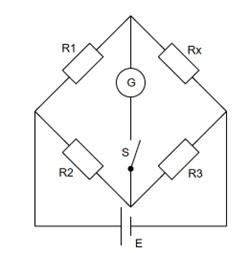
\includegraphics[width=0.35\textwidth]{demo.jpg}
\end{figure}

当电桥不平衡时，检流计中有电流通过，指针偏转。通过调节已知电阻，使得检流计指针回到零位，
使电桥达到平衡，根据平衡条件，必须满足：

\[
\frac{R_1}{R_x} = \frac{R_2}{R_3}
\]

因此得到待测电阻 $R_x$ 的测量公式：

\[
R_x = \frac{R_1 R_3}{R_2}
\]

以上是直接测量的方法，误差主要来源于已知电阻 $R_1$ 、$R_2$ 和 $R_3$ ，为了减小这种系统误差，
交换 $R_3$ 与 $R_x$ 的位置，并调节 $R_3$ 至 $R_3'$ 使得电桥再次达到平衡，此时满足：

\[
R_x = \frac{R_2 R_3'}{R_1}
\]

因此现在消除了已知电阻 $R_1$ 和 $R_2$ 的误差影响，待测电阻 $R_x$ 的测量公式为：

\[
R_x = \sqrt{R_3 \cdot R_3'}
\]

当电路中的电流非常小时，检流计可能还没有发生偏转，即电桥不够灵敏，对未知电阻的测量产生影响。
那么当 $\Delta R_3$ 为电阻箱 $R_3$ 的改变量，$\Delta d$ 为待测电阻的相对改变量引起的检流计指针偏转格数时，定量表示电桥灵敏度为：
\[
S = \frac{\Delta d}{\Delta R_3 / R_3}
\]

实验时，利用检流计、电阻箱、直流电源和待测电阻搭建惠斯登电桥，选取适当的比率臂，调节电阻箱阻值，开始时检流计指针有偏转，
随着调节电阻变化逐渐减小，直至回到零位。采用交换法减小误差，测量并记录多组数据，包括电桥的灵敏度。

此外，使用 $QJ-23$ 型盒式惠斯登电桥测量8个等值电阻，并计算它们的离散程度。

\subsection{实验重点（3分）}

本实验的学习重点在于了解惠斯登电桥的工作原理和特点，并掌握电桥的组装和用于测量未知电阻的方法，
掌握使用盒式惠斯登电桥测量电阻的方法，以及学习对测量结果进行误差分析的基本方法。

\subsection{实验难点（2分）}

本实验的实现难点主要在于对电桥平衡状态的精确判定上，检流计指针较灵敏，容易受环境干扰、电源波动等因素影响，
达到稳定平衡点的要求较高；而调节电阻不是连续变化的阻值，有精度上的限制。

\newpage
\section{原始数据（20分）}
实验测量数据：
\begin{figure}[htbp!]
    \centering
    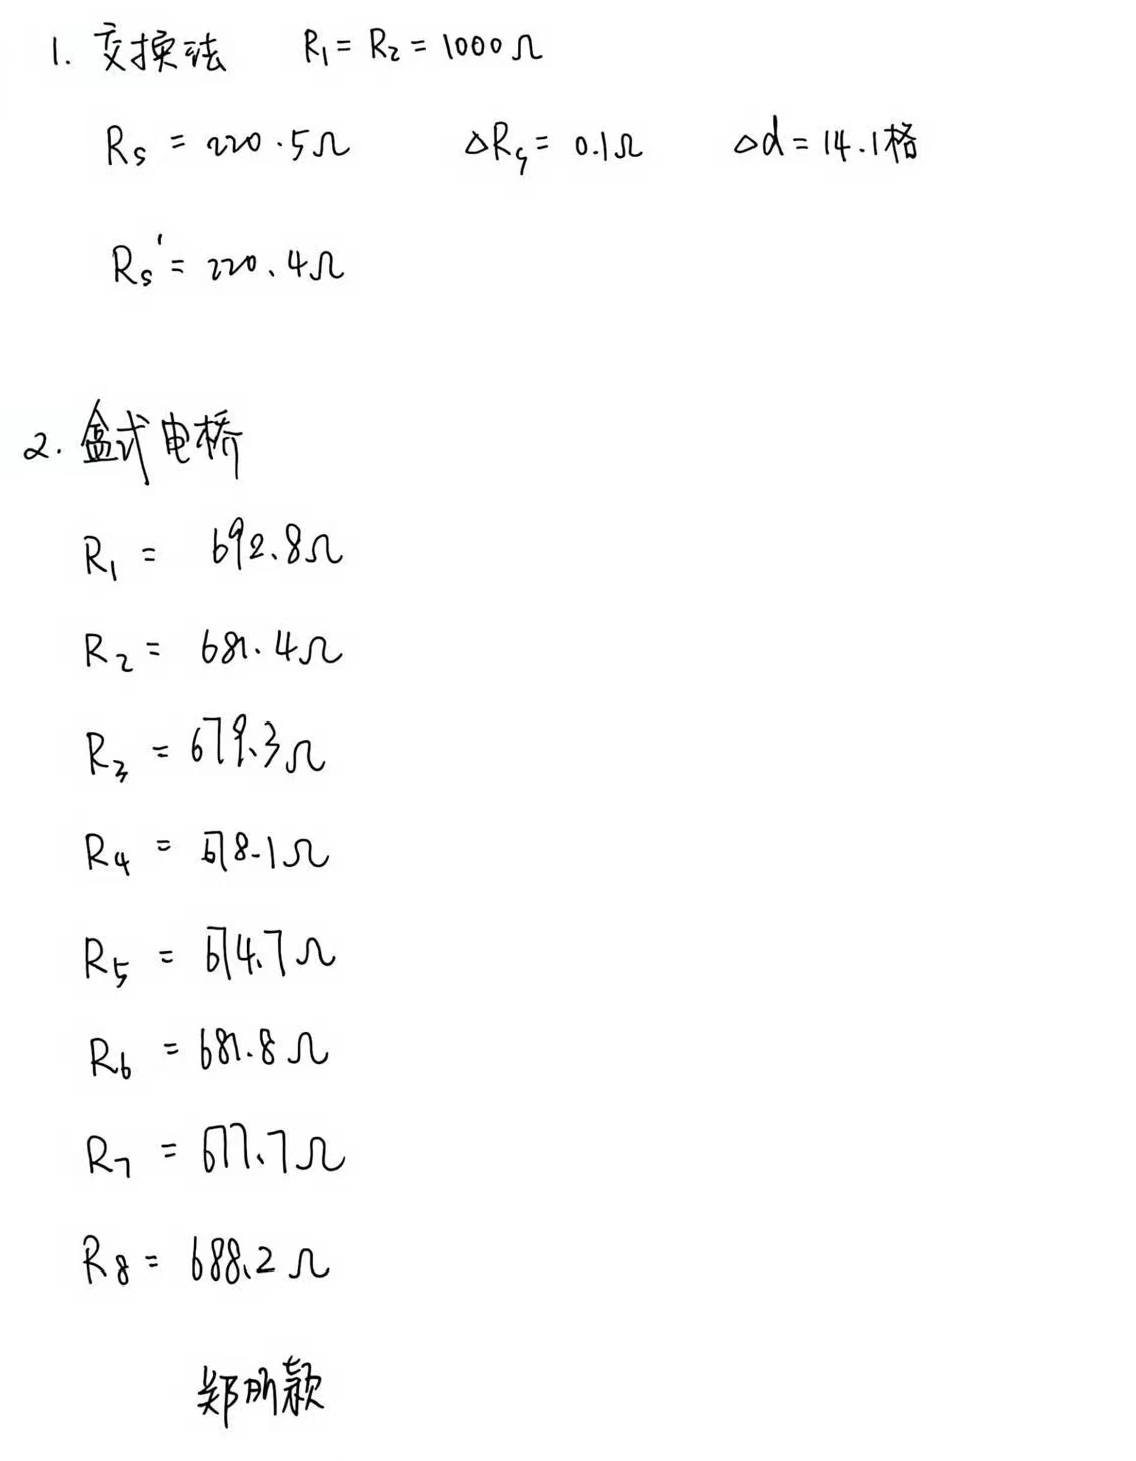
\includegraphics[width = 0.8\textwidth]{data.png}
\end{figure}

\FloatBarrier

\section{结果与分析（60分）}
\subsection{数据处理与结果（30分）}

\textbf{1. 自组电桥测未知电阻}

利用直流电源、检流计、电阻箱等组装惠斯登电桥，选择比率臂为 $\frac{R_1}{R_2} = \frac{1000 \Omega}{1000 \Omega} = 1$ 。

通过交换法测量未知电阻，交换前后分别有 $R_3 = 220.5 \Omega$ 和 $R_3' = 220.4 \Omega$ ，
因此得到未知电阻的值：
\[
\bar{R_x} = \sqrt{R_3 \cdot R_3'} = 220.4 \Omega
\]

通过交换法避免了 $R_1$ 和 $R_2$ 导致的误差后，还要考虑 $R_3$ 导致的误差：
\[
U(R_3) = \pm (a + b \cdot \frac{m}{R_3}) R_3 \% = \pm (0.001 R_3 + 0.012) = \pm 0.23 \Omega
\]

此外，由于电桥灵敏会引入不确定度，先测量电桥灵敏度，有 $\Delta R_3 = 0.1 \Omega$ ， $\Delta d = 14.1$ 格，因此：
\[
S = \frac{\Delta d}{\Delta R_3 / R_3} = 3.1 \times 10^4 \text{格} 
\]

这里用 $B$ 类不确定度替代待测电阻总的不确定度，满足：
\[
E = \frac{U(R_x)}{\bar{R_x}} = \sqrt{(0.001 + \frac{0.002m}{R_3})^2 + (\frac{0.2}{S})^2} = 0.11 \%
\]

因此得到待测电阻的不确定度 $U(R_x) = 0.2 \Omega$ ，最终待测电阻的结果为：
\[
R_x = \bar{R_x} \pm U(R_x) = (220.4 \pm 0.2) \Omega
\]

\textbf{2. 用盒式电桥测电阻的离散度}

用盒式电桥测量多个电阻的阻值：
\begin{table}[htbp!]
    \centering
    \begin{tabular}{c|cccccccc}
        \hline
        电阻 $R_i$ & $R_1$ & $R_2$ & $R_3$ & $R_4$ & $R_5$ & $R_6$ & $R_7$ & $R_8$ \\
        \hline
        阻值 $/ \Omega$ & 692.8 & 681.4 & 679.3 & 678.1 & 674.7 & 681.8 & 677.7 & 688.2 \\
        \hline
    \end{tabular}
\end{table}

\[
\bar{R_x} = \frac{1}{8} \sum_{i=1}^8 R_i = 681.8 \Omega
\]

此时 $n = 8$ ，计算标准偏差：
\[
s = \sqrt{\frac{1}{n - 1} \sum_{i=1}^{8} (R_i - \bar{R_x})^2} = 6.0 \Omega
\]

因此这些电阻的离散度为：
\[
\text{离散度} = \frac{s}{\bar{R_x}} \times 100 \% = 0.9 \%
\]

\subsection{误差分析（20分）}

在自组惠斯登电桥测量未知电阻的阻值时，通过交换法消除了桥臂上 $R_1$ 和 $R_2$ 造成的系统误差，
但是仍然有 $R_3$ 带来的误差。 $R_3$ 的最小分度值为 $0.1 \Omega$ ，
实际测量中发现这个最小改变量无法使检流计完全归零，即 $R_3$ 的调节精度不够高，
限制了未知电阻的测量精度。

在使用 $QJ-23$ 型盒式惠斯登电桥测量电阻时，由于这个电桥内置检流计和可调节电阻精度都不够高，
影响了未知电阻的测量精度。

此外，惠斯登电桥本身的灵敏度对测量结果有较大影响，灵敏度越高的电桥测量结果也就越准确。

\subsection{实验探讨（10分）}

本实验主要通过惠斯登电桥的平衡原理并结合误差控制方法测量未知电阻。
实验过程中，采用交换法有效消除了比率臂电阻引入的系统误差，提高了未知电阻测量的准确性；
通过测定电桥灵敏度并引入不确定度分析，使结果具有明确的定量误差范围。未知电阻的测量阻值与理论参考值符合较好，
误差分析表明测量精度较高，离散度计算表明8个电阻的一致性较好。


\section{思考题（10分）}

\textbf{1. 为什么用惠斯登电桥测电阻比伏安法测量的准确度高？用电桥法测电阻产生误差的主要因素是什么？}

惠斯登电桥属于零位比较测量法，在电桥达到平衡时，检流计中无电流通过，测量结果只与各桥臂电阻的比值有关，
而与电源电压的稳定性、检流计内阻以及导线电阻等因素基本无关，并且通过交换法已经消除了比率臂上电阻的误差。
相比之下，伏安法需要同时测量电压和电流，电压表和电流表本身的内阻、量程误差以及电源波动都会直接引入系统误差。
因此，在相同实验条件下，惠斯登电桥具有更高的测量精度和稳定性。

用电桥法测量电阻的主要误差来源包括桥臂电阻本身的误差和接触电阻，电桥灵敏度有限导致平衡状态判断不够精确，
检流计零点漂移及环境干扰。


\textbf{2. 为了提高电桥测量灵敏度，应采取哪些措施？为什么？}

首先，合理选择比率臂，尽量使四个桥臂电阻处于同一数量级，且待测电阻接近平衡状态，因为此时电桥对电阻微小变化最为敏感。
其次，适当提高电源电压，在不引起电阻发热和仪表超过量程的前提下增大电路中电流，从而增强检流计的偏转响应。
再次，选用灵敏度更高、内阻合适的检流计，并尽量减小接触电阻和导线电阻对测量的影响。
此外，选用最小分度值更小的电阻箱，使得电桥平衡的调节更准确。

\textbf{3. 用电桥测电阻时，若线路接通后检流计指针总是往一个方向偏转或总不偏转，试分析是什么原因？}

用惠斯登电桥测量电阻时，若接通线路后检流计指针总是向同一方向偏转，通常说明电桥始终处于不平衡状态，
可能是比率臂或比较臂电阻选择不当，使待测电阻与电桥参数相差过大而无法调节平衡；也可能电桥接线错误，
或者桥臂中存在接触不良或元件损坏，出现短路或断路。

若检流计指针始终不发生偏转，可能是电桥接线有误，如电源未接通、电路存在断路、检流计短路；
也可能是检流计灵敏度过低或量程选择不当，使微小电流无法被指示。

\textbf{4. 惠斯登电桥比率臂选取的原则是什么？为什么要这样选取？}

选取惠斯登电桥的比率臂时，应在电阻箱不超过最大阻值的前提下使比率臂接近待测电阻与比较电阻之比，
并尽量使电桥在平衡时各桥臂电阻处于同一数量级。

这样选取的原因在于，当四个桥臂阻值相近时，电桥的灵敏度最高，检流计对电阻微小变化的响应更明显，
有利于准确判断平衡状态；同时可以避免某一桥臂电流过大或过小，从而减小接触电阻、导线电阻及仪表误差的相对影响，
提高测量精度和稳定性；还可以尽可能多地使用电阻箱的位数，提高结果的测量精度。

\textbf{5. 如何使用自组电桥测量电表内阻（注意电表所能允许通过的最大电流）？根据电桥平衡特点，可否将桥路中的检流计去掉，换成行测电表判别电桥的平衡？}

使用自组惠斯登电桥测量电表内阻时，将被测电表作为待测电阻接入桥臂之一，并在电路中串联限流电阻或选用较低电源电压，
使通过电表的电流始终小于其允许的最大电流，防止超出量程。实验过程中，通过调节比较臂电阻，使电桥达到平衡状态；
当检流计指示为零时，根据电桥平衡条件即可计算出电表的内阻。

根据惠斯登电桥的平衡特点，理论上可以去掉检流计，只要接通原含检流计的线路前后行测电表示数不改变，就说明电桥平衡。
但是由于行测电表精度较低，难以检测微小电流变化，所以实际上它的示数不改变不一定说明电桥仍然平衡，误差可能较大。

\begin{thebibliography}{9}
    \bibitem{ref1}
    刘凤智. 惠斯登电桥比例臂的选取[J]. 科技风,2018(23):210,213. DOI:10.19392/j.cnki.1671-7341.201823190. 
    
    \bibitem{ref2}
    李伟,陈红斌. 惠斯登电桥测量灵敏度分析[J]. 科技视界,2015(30):172,168. DOI:10.3969/j.issn.2095-2457.2015.30.126. 

\end{thebibliography}

\input{注意事项}
\end{document}
